%%%%%%%%%%%%%%%%%%%%%%%%%%%%%%%%%%%%%%%%%%%%%%%%%%%%%%%%%%%%%%%%%%%%%%%%%%%%%%%%%%%%%%%%%%%%%%
%%%%%%%%%%%%%%%%%%%%%%%%%%%%%%%%%%%%%%%%%%%%%%%%%%%%%%%%%%%%%%%%%%%%%%%%%%%%%%%%%%%%%%%%%%%%%%
%%%%%%%%%%% GPU
%%%%%%%%%%%%%%%%%%%%%%%%%%%%%%%%%%%%%%%%%%%%%%%%%%%%%%%%%%%%%%%%%%%%%%%%%%%%%%%%%%%%%%%%%%%%%%
%%%%%%%%%%%%%%%%%%%%%%%%%%%%%%%%%%%%%%%%%%%%%%%%%%%%%%%%%%%%%%%%%%%%%%%%%%%%%%%%%%%%%%%%%%%%%%


% \cleardoublepage
\chapter{Signal Processing with GPUs}
\label{sec:gpu}

This thesis explores the use of GPUs in data-aided estimation, equalization and filtering operations.

A Graphics Processing Unit (GPU) is a computational unit with a highly-parallel architecture well-suited for executing the same function on many data elements.
In the past, GPUs were used to process graphics data.
Recently, general purpose GPUs are being used for high performance computing in computer vision, deep learning, artificial intelligence and signal processing \cite{wikipedia-gpu:2015}.

GPUs cannot be programmed the way as a CPU. 
NVIDIA released a extension to C, C++ and Fortran called CUDA (Compute Unified Device Architecture).
CUDA allows a programmer to write C++ like functions that are massively parallel called \textit{kernels}.
To invoke parallelism, a GPU kernel is called $N$ times and mapped to $N$ \textit{threads} that run concurrently.
To achieve the full potential of high performance GPUs, kernels must be written with some basic concepts about GPU architecture and memory in mind.

The purpose of this overview is to provide context for the contributions of this thesis.
As such this overview is not a tutorial.
For a full explination of CUDA programming please see the CUDA toolkit documentation \cite{CUDA_toolkit_doc}.

\section{Simple GPU code example}
If a programmer has some C++ experience, learning how to program GPUs using CUDA comes fairly easily.
GPU code still runs top to bottom and memory still has to be allocated.
The only real difference is where the memory physically is and how functions run on GPUs.
To run functions or kernels on GPUs, the memory must be copied from the host (CPU) to the device (GPU).
Once the memory has been copied, the parallel GPU kernels can be called.
After the GPU kernels have finished, the resulting memory has to be copied back from the device (GPU) to the host (CPU).

Listing \ref{code:GPUvsCPU} shows a simple program that sums to vectors together
\begin{equation}
\begin{matrix}
\mathbf{C}_1 = \mathbf{A}_1 + \mathbf{B}_1 \\
\mathbf{C}_2 = \mathbf{A}_2 + \mathbf{B}_2
\end{matrix}
\end{equation}
where each vector is length $1024$.
Figure \ref{fig:CPUaddBlockDiagram} shows how the CPU computes $\mathbf{C}_1$ by summing elements of $\mathbf{A}_1$ and $\mathbf{B}_1$ together \textit{sequentially}.
Figure \ref{fig:GPUaddBlockDiagram} shows how the GPU computes $\mathbf{C}_2$ by summing elements of $\mathbf{A}_1$ and $\mathbf{B}_1$ together \textit{in parallel}.
The GPU kernel computes every element of $\mathbf{C}_2$ in parallel while the CPU computes one element of $\mathbf{C}_1$ at a time.
\begin{figure}
	\centering\includegraphics[width=3.17in/100*55]{figures/gpu_intro/CPUaddBlockDiagram.pdf}
	\caption{A block diagram of how a CPU sequentially performs vector addition.}
	\label{fig:CPUaddBlockDiagram}
\end{figure}
\begin{figure}
	\centering\includegraphics[width=4.69in/100*55]{figures/gpu_intro/GPUaddBlockDiagram.pdf}
	\caption{A block diagram of how a GPU performs vector addition in parallel.}
	\label{fig:GPUaddBlockDiagram}
\end{figure}
\singlespacing
\clearpage
\begin{lstlisting}[caption={Comparison of CPU verse GPU code.},label={code:GPUvsCPU}]
#include <iostream>
#include <stdlib.h>
#include <math.h>
using namespace std;

void VecAddCPU(int* destination,int* source0,int* source1,int myLength){
	for(int i = 0; i < myLength; i++)
		destination[i] = source0[i] + source1[i];
}

__global__ void VecAddGPU(int* destination, int* source0, int* source1, int lastThread){
	int i = blockIdx.x*blockDim.x + threadIdx.x;

	// don't access elements out of bounds
	if(i >= lastThread)
		return;

	destination[i] = source0[i] + source1[i];
}

int main(){
	int numPoints = pow(2,22);
	cout << numPoints << endl;
	/*--------------------------------------------------------------------
                               	   CPU Start
	--------------------------------------------------------------------*/
	// allocate memory on host
	int *A1;
	int *B1;
	int *C1;
	A1 = (int*) malloc (numPoints*sizeof(int));
	B1 = (int*) malloc (numPoints*sizeof(int));
	C1 = (int*) malloc (numPoints*sizeof(int));

	// Initialize vectors 0-99
	for(int i = 0; i < numPoints; i++){
		A1[i] = rand()%100;
		B1[i] = rand()%100;
	}

	// vector sum C1 = A1 + B1
	VecAddCPU(C1, A1, B1, numPoints);
	/*--------------------------------------------------------------------
                               	   CPU End
	--------------------------------------------------------------------*/

	/*--------------------------------------------------------------------
                               	   GPU End
	--------------------------------------------------------------------*/
	// allocate memory on host for result
	int *C2;
	C2 = (int*) malloc (numPoints*sizeof(int));

	// allocate memory on device for computation
	int *A2_gpu;
	int *B2_gpu;
	int *C2_gpu;
	cudaMalloc(&A2_gpu, sizeof(int)*numPoints);
	cudaMalloc(&B2_gpu, sizeof(int)*numPoints);
	cudaMalloc(&C2_gpu, sizeof(int)*numPoints);

	// Copy vectors A and B from host to device
	cudaMemcpy(A2_gpu, A1, sizeof(int)*numPoints, cudaMemcpyHostToDevice);
	cudaMemcpy(B2_gpu, B1, sizeof(int)*numPoints, cudaMemcpyHostToDevice);

	// Set optimal number of threads per block
	int numTreadsPerBlock = 32;

	// Compute number of blocks for set number of threads
	int numBlocks = numPoints/numTreadsPerBlock;

	// If there are left over points, run an extra block
	if(numPoints % numTreadsPerBlock > 0)
		numBlocks++;

	// Run computation on device
	//for(int i = 0; i < 100; i++)
		VecAddGPU<<<numBlocks, numTreadsPerBlock>>>(C2_gpu, A2_gpu, B2_gpu, numPoints);

	// Copy vector C2 from device to host
	cudaMemcpy(C2, C2_gpu, sizeof(int)*numPoints, cudaMemcpyDeviceToHost);
	/*--------------------------------------------------------------------
                               	   GPU End
	--------------------------------------------------------------------*/

	// Free vectors on CPU
	free(A1);
	free(B1);
	free(C1);
	free(C2);

	// Free vectors on GPU
	cudaFree(A2_gpu);
	cudaFree(B2_gpu);
	cudaFree(C2_gpu);
}
\end{lstlisting}
\doublespacing

\section{GPU kernel using threads and thread blocks}
A GPU kernel is executed on a GPU by launching numTreadsPerBlock$\times$numBlocks 
threads.
Each thread has a unique index.
CUDA calls this indes threadIdx and blockIdx.
threadIdx is the thread index inside the assigned thread block.
blockIdx is the index of the block the thread is assigned.
blockDim is the number of threads assigned per block, in fact blockDim $=$ numTreadsPerBlock.
Both threadIdx and blockIdx are three dimensional and have x, y and z components.
In this thesis only the x dimension is used because GPU kernels operate only on vectors.

To replace a CPU for loop that runs $0$ to $N-1$, a GPU kernel launches $N$ threads are with $T$ threads per thread block.
The number of blocks need is $M = \frac{N}{T}$ or $M = \frac{N}{T}+1$ if $N$ is not an integer multiple of $T$.
Figure \ref{fig:threadsBlocks32} shows $32$ threads launched in $4$ thread blocks with $8$ threads per block.
Figure \ref{fig:threadsBlocks36} shows $36$ threads launched in $5$ thread blocks with $8$ threads per block. An full extra thread block must be launched to with $8$ threads but $4$ threads are idle.
\begin{figure}
	\centering\includegraphics[width=4in/100*55]{figures/gpu_intro/threadsBlocks32.pdf}
	\caption{Block $0$ $32$ threads launched in $4$ thread blocks with $8$ threads per block.}
	\label{fig:threadsBlocks32}
\end{figure}
\begin{figure}
	\centering\includegraphics[width=5in/100*55]{figures/gpu_intro/threadsBlocks36.pdf}
	\caption{$36$ threads launched in $5$ thread blocks with $8$ threads per block with $4$ idle threads.}
	\label{fig:threadsBlocks36}
\end{figure}

\section{GPU memory}
Thread blocks run independent of other thread blocks.
The GPU does not guarantee Block $0$ will execute before Block $2$.
Threads in blocks can coordinate and use shared memory but blocks do not coordinate with other blocks.
Threads have access to private local memory that is fast and efficient.
Each thread in a thread block has access to private shared memory in the thread block.
All threads have access to global memory.

Local memory is the fastest and global memory is by far the slowest.
One global memory access takes 400-800 clock cycles while a local memory is a few clock cycles.
Why not just do all computations in local memory?
The memory needs come from global memory to before it can be used in local memory.
Memory should be saved in shared memory if many threads are going to use it in a thread block.
Local and shared memory should be used as much as possible but sometimes a GPU kernel cant utilized local and shared memory because elements might only be used once.
\begin{sidewaysfigure}
	\centering\includegraphics[width=9in/100*55]{figures/gpu_intro/fullGPUmemBlockDiagram.png}
	\caption{A block diagram where local, shared, and global memory is located. Each thread has private local memory. Each thread block has private shared memory. The GPU has global memory that all threads can access.}
	\label{fig:fullGPUmemBlockDiagram}
\end{sidewaysfigure}

Why is global memory so slow?
Looking at the physical hardware will shed some light.
This thesis uses NVIDIA Tesla K40c and K20c GPUs, Table \ref{tab:gpu-resources_jeffs} gives some specifications and Figure \ref{fig:GPUpicture} shows the form factor of the these GPUs.
The red box in Figure \ref{fig:GPUarch} show the GPU chip and the yellow boxes show the SRAM that is \textit{off} the GPU chip.
The GPU global memory is located in the SRAM.
To move memory to thread blocks \textit{on} the GPU chip from global memory requires fetching memory from \textit{off} the GPU.
Now 400-800 clock cycles doesn't sound all the bad huh?
\begin{figure}
	\centering\includegraphics[width=5in]{figures/gpu_intro/k40c_k20c.jpg}
	\caption{NVIDIA Tesla K40c and K20c.}
	\label{fig:GPUpicture}
\end{figure}
\begin{figure}
	\centering\includegraphics[width=\textwidth]{figures/gpu_intro/Kepler_box.png}
	\caption{Example of an NVIDIA GPU card. The SRAM is shown to be boxed in yellow. The GPU chip is shown to be boxed in red.}
	\label{fig:GPUarch}
\end{figure}
\begin{table}
\begin{center}
\begin{tabular}{lll}
	\toprule
	Feature 			& Tesla K40c 	& Tesla K20c 	\\ \midrule
	Memory size (GDDR5) & 12 GB 		& 5 GB 			\\
	CUDA cores 			& 2880 			& 2496 			\\
	Base clock (MHz) 	& 745 			& 732 			\\ \bottomrule
\end{tabular}
\end{center}
\caption{The computational resources available with three NVIDIA GPUs used in this thesis (1x Tesla K40c 2x Tesla K20c).}
\label{tab:gpu-resources_jeffs}
\end{table}

\section{Cuda Libraries}
CUDA isn't just a programming language, it also has many libraries that are extreemly useful that are optimized for NVIDIA GPUs.
CUDA libraries are written by NVIDIA engineers that know how to squeeze out every drop of performance out of NVIDIA GPUs.
Because ninjas are unbeatable, NVIDIA engineers are known as ninjas in the Telemetry Group at BYU.
While figuring out how to optimize a GPU kernel is extremely satisfying, GPU programmers should always search the CUDA libraries for any thing that might be useful.

Some libraries used in this Thesis are
\begin{itemize}
  \item cufft
  \item cublas
  \item cusolver
  \item cusolverSp
\end{itemize}

\section{Cuda Convolution}
An important tool to Digital Communications and Digital Signal Processing is convolution.
Time domain convolution is
\begin{align}
y(n) = \sum^{L_\text{h}-1}_{m=0} x(m) h(n-m)
	 \label{eq:simple_conv}
\end{align}
where $x(m)$, $h(n-m)$ and $y(n)$ are complex. 
While Listing \ref{code:GPUvsCPU} is a simple and good example showing how program GPUs, frankly, it is pretty boring and doesn't display the real challenges and tradeoffs of GPUs.
Listing \ref{code:convFun} shows four different ways of implementing convolution
\begin{itemize}
  \item time domain convolution in a CPU
  \item time domain convolution in a GPU using global memory
  \item time domain convolution in a GPU using shared memory
  \item frequency domain convolution in a GPU using CUDA libraries
\end{itemize}
The CPU implements Equation \eqref{eq:simple_conv} in ConvCPU directly from line $6$ to $30$.
The GPU implements time domain convolution using global memory in the GPU kernel ConvGPU.
ConvGPU on lines $32$ to $59$ is a parallel of ConvCPU.
ConvGPU implements time domain convolution by accessing global memory for any needed element of the signal and filter.

Threads accessing the same elements of the filter in global memory seems like a waste of valuable clock cycles.
The GPU kernel ConvGPUshared on lines $61$ to $96$ differs slightly from ConvGPU by making $L_\text{h}$ threads save the filter to shared memory from global memory.

Any graduate of a signal processing class knows the trade off of convolution in the time verse frequency domain.
Time domain convolution takes $\approx L_\text{s} L_\text{h}$ complex multiplies where $L_\text{s}$ is the signal length and $L_\text{h}$ is the filter length.
Frequency domain convolution takes $\approx \frac{3 N_\text{FFT}}{2} \log_2(N_\text{FFT}) + N_\text{FFT}$ complex multiplies where $N_\text{FFT}$ is the next multiple of $2$ above the convolution length $L_\text{s}+L_\text{h}-1$.

Lines $213$ to $232$ show how to do frequency domain convolution using the cuFFT library.

So the questions are:
When should I stay on the host and run my convolution on the CPU?
When should I copy my vectors to the GPU, run my convolution, then copy the vectors back to the host?
If I am going to run my convolution the GPU, when should I only use global memory?
When should I use shared memory?
When should I do convolution in the frequency domain?

The answer to all of the questions is...it depends on your signal length, filter length, CPU, GPU and memory.

The CUDA programmer can make an educated guess on which way will be fastest, but until the computations have been done in the GPU there is no definite answer.
Figure \ref{fig:CPUvsGPU} shows a comparison of computation time by varying the signal length with a set filter length.
The signal length is varied from $1$ to $~50000$ and the filter length is $186$;
The functions in \ref{code:GPUvsCPU} where ran on a NVIDIA Tesla K40c GPU.
Judging my the Figure, for signals of any significnt length, GPU convolution is much faster than CPU.
\begin{figure}
	\centering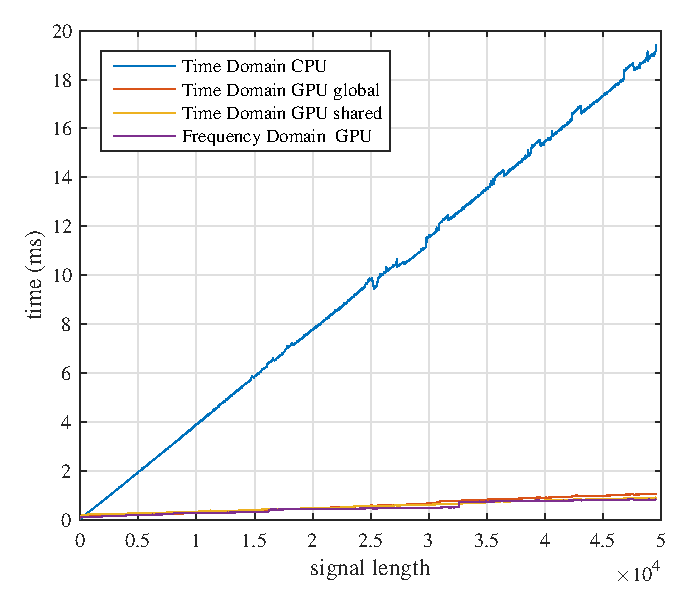
\includegraphics[width=4in]{figures/gpu_intro/CPUvsGPU.eps}
	\caption{Comparison of complex convolution in on CPU to GPU with varying signal lengths.}
	\label{fig:CPUvsGPU}
\end{figure}

Is it ever better to do convolution on the CPU rather than GPU?
Yes, but for very short signals with a $186$ tap filter.
Figure \ref{fig:CPUvsGPU_CPUtoGPU} shows when a CPU is faster than a GPU.
\begin{figure}
	\centering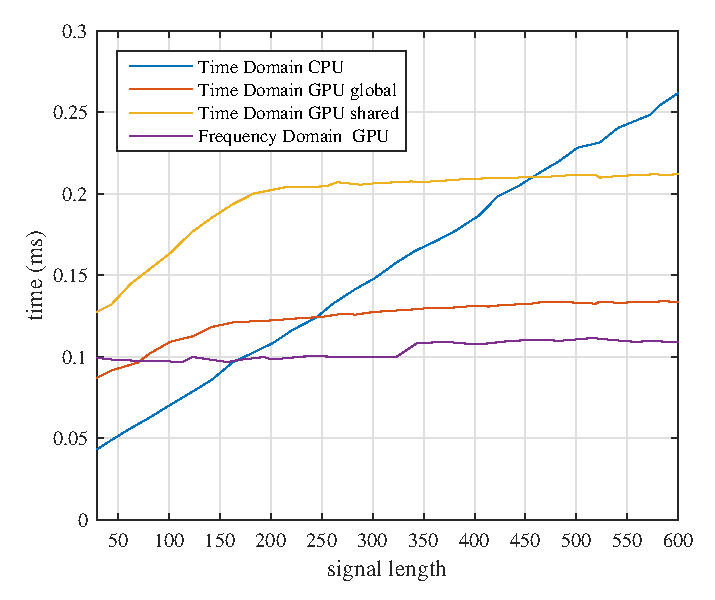
\includegraphics[width=4in]{figures/gpu_intro/CPUvsGPU_CPUtoGPU.eps}
	\caption{Plot showing when CPU convolution is faster than GPU convolution.}
	\label{fig:CPUvsGPU_CPUtoGPU}
\end{figure}

Now for the interesting question, if I am going to do convolution in the GPU, should I do time domain or frequency domain convolution?
If I do time domain convolution, should I use global or shared memory?
Figure \ref{fig:CPUvsGPU_GPUtoGPU} shows that the answer is, ``it depends''.
A good choice is to do frequency domain, but not always.
As the signal length increases, the frequency domain execution time has steps because the signal is zero padded out to the next power of 2 to leverage the Cooley-Tukey FFT algorithm \cite{Cooley-Tukey_old}.
\begin{figure}
	\centering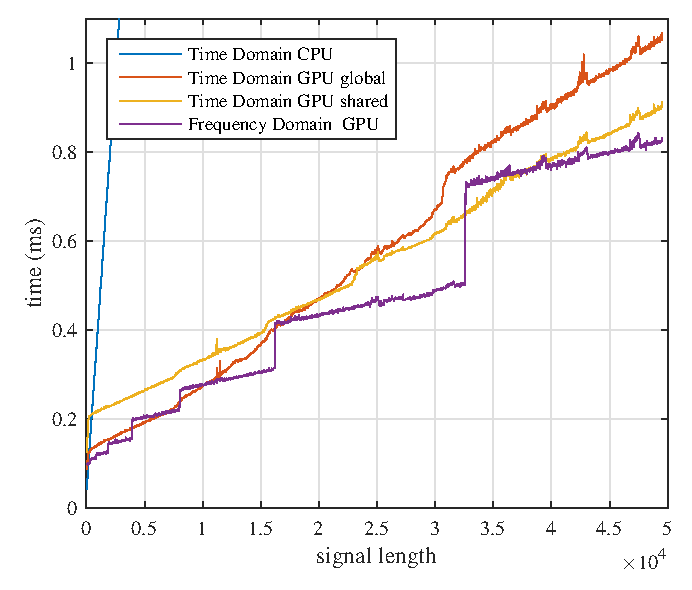
\includegraphics[width=4in]{figures/gpu_intro/CPUvsGPU_GPUtoGPU.eps}
	\caption{Plot showing trade offs with convolution in GPUs.}
	\label{fig:CPUvsGPU_GPUtoGPU}
\end{figure}

Usually, when implementing convolution, the signal and filter length is set.
If is good practice to implement convolution in the CPU and GPU in many ways to evaluate which way is best.
Choosing the signal length to be $2^{15}$ and the filter length to be $186$, Table \ref{tab:CPUvsGPUtable} shows how the different algorithms compare.
\begin{table}
\begin{center}
\begin{tabular}{lll}
	\toprule
	Algorithm 								& time (ms) \\ \midrule
	CPU time domain (ConvCPU) 				& 131.943 	\\
	GPU time domain global (ConvGPU) 		& 7.79477	\\
	GPU time domain shared (ConvGPUshared) 	& 6.77736	\\
	GPU frequency domain shared 			& 5.81085	\\ 
	\bottomrule
\end{tabular}
\end{center}
\caption{Convolution computation times with signal length $2^{15} = 32768$ and filter length $186$ on a Tesla K40c GPU.}
\label{tab:CPUvsGPUtable}
\end{table}




\section{Thread Optimization}
When first introduced to GPUs, a programmer might to tempted to launch as many threads per block possible.
But, notice in Listing \ref{code:convFun} lines $190$, $203$, $219$ and $225$ launch a minimum of $96$ threads per block and maximum of $192$ threads per block.
Running the GPU at lower occupancy leaves each thread with more resources and memory bandwidth.
If $1024$ threads per block were always launched, lighter computaion GPU kernels will be starving for memory while other thread blocks eat up the memory bandwidth.

Improving memory accesses should always be the first optimization when a GPU kernel needs to be faster.
The next step is to find the optimal number of threads per block to launch.
The number of threads per block affect the amount of resources available to each thread.
If a kernel is more computationally heavy, launching less threads per block may lead to faster execution time because threads have more resources available. 

Knowing the perfect number of threads per block to launch is challenging to calculate.
Luckily, there is a finite number of possible threads per block, $1$ to $1024$.
A simple test program could time a GPU kernel while sweeping the number of threads per block from $1$ to $1024$.
The number of threads per block with the fastest computation time is the optimal number of threads per block for that specific GPU kernel.

Most of the time the optimal number of threads per block is a multiple of $32$. 
At the lowest level of architecture, GPU do computations in \textit{warps}.
Warps are groups of $32$ threads to do every computation together in lock step.
If the number of threads per block is a non multiple of $32$, some threads in a warp will be idle and the GPU will be wasting resources.

Figure \ref{fig:threadOptimzation_ConvGPU} shows the execution time of ConvGPU while varying threads per block.
The minimum execution time is $651651$ at $128$ threads per block.










\singlespacing
\clearpage
\begin{lstlisting}[caption={CUDA code to performing complex convolution four different ways: time domain CPU, time domain GPU, time domain GPU using shared memory and frequency domain GPU.},label={code:convFun}]
#include <cufft.h>
using namespace std;
// Length of Filter (186 is a magic number)
const int LH = 186;

void ConvCPU(cufftComplex* y,cufftComplex* x,cufftComplex* h,int Lx,int Lh){
	for(int yIdx = 0; yIdx < Lx+Lh-1; yIdx++){
		cufftComplex temp;
		temp.x = 0;
		temp.y = 0;
		for(int hIdx = 0; hIdx < Lh; hIdx++){
			int xAccessIdx = yIdx-hIdx;
			if(xAccessIdx>=0 && xAccessIdx<Lx){
				// temp += x[xAccessIdx]*h[hIdx];
				// (A+jB)(C+jD) = (AC-BD) + j(AD+BC)
				float A = x[xAccessIdx].x;
				float B = x[xAccessIdx].y;
				float C = h[hIdx].x;
				float D = h[hIdx].y;
				cufftComplex complexMult;
				complexMult.x = A*C-B*D;
				complexMult.y = A*D+B*C;

				temp.x += complexMult.x;
				temp.y += complexMult.y;
			}
		}
		y[yIdx] = temp;
	}
}

__global__ void ConvGPU(cufftComplex* y,cufftComplex* x,cufftComplex* h,int Lx,int Lh){
	int yIdx = blockIdx.x*blockDim.x + threadIdx.x;
	int lastThread = Lx+Lh-1;
	// Don't access elements out of bounds
	if(yIdx >= lastThread)
		return;
	cufftComplex temp;
	temp.x = 0;
	temp.y = 0;
	for(int hIdx = 0; hIdx < Lh; hIdx++){
		int xAccessIdx = yIdx-hIdx;
		if(xAccessIdx>=0 && xAccessIdx<Lx){
			// temp += x[xAccessIdx]*h[hIdx];
			// (A+jB)(C+jD) = (AC-BD) + j(AD+BC)
			float A = x[xAccessIdx].x;
			float B = x[xAccessIdx].y;
			float C = h[hIdx].x;
			float D = h[hIdx].y;
			cufftComplex complexMult;
			complexMult.x = A*C-B*D;
			complexMult.y = A*D+B*C;

			temp.x += complexMult.x;
			temp.y += complexMult.y;
		}
		y[yIdx] = temp;
	}
}

__global__ void ConvGPUshared(cufftComplex* y,cufftComplex* x,cufftComplex* h,int Lx,int Lh){
	int yIdx = blockIdx.x*blockDim.x + threadIdx.x;
	// Be sure to read in full h_shared before checking lastThread
	// First Lh threads in thread block read h from global memory into shared memory
	__shared__ cufftComplex h_shared[LH];
	if(threadIdx.x < LH)
		h_shared[threadIdx.x] = h[threadIdx.x];
	int lastThread = Lx+Lh-1;
	// Don't access elements out of bounds
	if(yIdx >= lastThread)
		return;
	// Thread barrier, ensures threads wait until h has been read into h_shared
	__syncthreads();
	cufftComplex temp;
	temp.x = 0;
	temp.y = 0;
	for(int hIdx = 0; hIdx < Lh; hIdx++){
		int xAccessIdx = yIdx-hIdx;
		if(xAccessIdx>=0 && xAccessIdx<Lx){
			// temp += x[xAccessIdx]*h_shared[hIdx];

			// (A+jB)(C+jD) = (AC-BD) + j(AD+BC)
			float A = x[xAccessIdx].x;
			float B = x[xAccessIdx].y;
			float C = h_shared[hIdx].x;
			float D = h_shared[hIdx].y;
			cufftComplex complexMult;
			complexMult.x = A*C-B*D;
			complexMult.y = A*D+B*C;

			temp.x += complexMult.x;
			temp.y += complexMult.y;
		}
		y[yIdx] = temp;
	}
}

__global__ void PointToPointMultiply(cufftComplex* vec0, cufftComplex* vec1, int lastThread){
	int i = blockIdx.x*blockDim.x + threadIdx.x;
	// Don't access elements out of bounds
	if(i >= lastThread)
		return;
	// vec0[i] = vec0[i]*vec1[i]];
	// (A+jB)(C+jD) = (AC-BD) + j(AD+BC)
	float A = vec0[i].x;
	float B = vec0[i].y;
	float C = vec1[i].x;
	float D = vec1[i].y;
	cufftComplex complexMult;
	complexMult.x = A*C-B*D;
	complexMult.y = A*D+B*C;
	vec0[i] = complexMult;
}

__global__ void ScalarMultiply(cufftComplex* vec0, float scalar, int lastThread){
	int i = blockIdx.x*blockDim.x + threadIdx.x;
	// Don't access elements out of bounds
	if(i >= lastThread)
		return;
	cufftComplex scalarMult;
	scalarMult.x = vec0[i].x*scalar;
	scalarMult.y = vec0[i].y*scalar;
	vec0[i] = scalarMult;
}

int main(){
	int mySignalLength = pow(2,15);
	int myFilterLength = LH;
	int myConvLength   = mySignalLength + myFilterLength - 1;
	int Nfft        = pow(2, ceil(log(myConvLength)/log(2)));
	int numTreadsPerBlock;
	int numBlocks;

	cufftHandle plan;
	int n[1] = {Nfft};
	cufftPlanMany(&plan,1,n,NULL,1,1,NULL,1,1,CUFFT_C2C,1);

	// Allocate memory on host
	cufftComplex *mySignal1;
	cufftComplex *myFilter1;
	cufftComplex *myConv1;
	cufftComplex *myConv2;
	cufftComplex *myConv3;
	cufftComplex *myConv4;
	mySignal1      = (cufftComplex*) malloc(mySignalLength*sizeof(cufftComplex));
	myFilter1      = (cufftComplex*) malloc(myFilterLength*sizeof(cufftComplex));
	myConv1        = (cufftComplex*) malloc(myConvLength  *sizeof(cufftComplex));
	myConv2        = (cufftComplex*) malloc(myConvLength  *sizeof(cufftComplex));
	myConv3        = (cufftComplex*) malloc(myConvLength  *sizeof(cufftComplex));
	myConv4        = (cufftComplex*) malloc(Nfft       *sizeof(cufftComplex));
	for(int i = 0; i < mySignalLength; i++){
		mySignal1[i].x = rand()%100-50;
		mySignal1[i].y = rand()%100-50;
	}
	for(int i = 0; i < myFilterLength; i++){
		myFilter1[i].x = rand()%100-50;
		myFilter1[i].y = rand()%100-50;
	}

	// Allocate memory on device
	cufftComplex *dev_mySignal2;
	cufftComplex *dev_myFilter2;
	cufftComplex *dev_myConv2;
	cufftComplex *dev_mySignal3;
	cufftComplex *dev_myFilter3;
	cufftComplex *dev_myConv3;
	cufftComplex *dev_mySignal4;
	cufftComplex *dev_myFilter4;
	cufftComplex *dev_myConv4;
	cudaMalloc(&dev_mySignal2, mySignalLength*sizeof(cufftComplex));
	cudaMalloc(&dev_myFilter2, myFilterLength*sizeof(cufftComplex));
	cudaMalloc(&dev_myConv2,   myConvLength  *sizeof(cufftComplex));
	cudaMalloc(&dev_mySignal3, mySignalLength*sizeof(cufftComplex));
	cudaMalloc(&dev_myFilter3, myFilterLength*sizeof(cufftComplex));
	cudaMalloc(&dev_myConv3,   myConvLength  *sizeof(cufftComplex));
	cudaMalloc(&dev_mySignal4, Nfft          *sizeof(cufftComplex));
	cudaMalloc(&dev_myFilter4, Nfft          *sizeof(cufftComplex));
	cudaMalloc(&dev_myConv4,   Nfft          *sizeof(cufftComplex));

	/*---------------------------------------------------------------------------------------
                                CPU Time Domain Direct Convolution
	---------------------------------------------------------------------------------------*/
	ConvCPU(myConv1,mySignal1,myFilter1,mySignalLength,myFilterLength);

	/*---------------------------------------------------------------------------------------
                                GPU Time DomainDirect Convolution
	---------------------------------------------------------------------------------------*/
	cudaMemcpy(dev_mySignal2, mySignal1, sizeof(cufftComplex)*mySignalLength, cudaMemcpyHostToDevice);
	cudaMemcpy(dev_myFilter2, myFilter1, sizeof(cufftComplex)*myFilterLength, cudaMemcpyHostToDevice);
	numTreadsPerBlock = 128;
	numBlocks = myConvLength/numTreadsPerBlock;
	if(myConvLength % numTreadsPerBlock > 0)
		numBlocks++;
	ConvGPU<<<numBlocks, numTreadsPerBlock>>>(dev_myConv2, dev_mySignal2, dev_myFilter2, mySignalLength, myFilterLength);
	cudaMemcpy(myConv2, dev_myConv2, myConvLength*sizeof(cufftComplex), cudaMemcpyDeviceToHost);


	/*---------------------------------------------------------------------------------------
                                GPU Time Domain Convolution Using Shared Memory
	---------------------------------------------------------------------------------------*/
	cudaMemcpy(dev_mySignal3, mySignal1, sizeof(cufftComplex)*mySignalLength, cudaMemcpyHostToDevice);
	cudaMemcpy(dev_myFilter3, myFilter1, sizeof(cufftComplex)*myFilterLength, cudaMemcpyHostToDevice);
	numTreadsPerBlock = 192;
	numBlocks = myConvLength/numTreadsPerBlock;
	if(myConvLength % numTreadsPerBlock > 0)
		numBlocks++;
	ConvGPUshared<<<numBlocks, numTreadsPerBlock>>>(dev_myConv3, dev_mySignal3, dev_myFilter3, mySignalLength, myFilterLength);
	cudaMemcpy(myConv3, dev_myConv3, myConvLength*sizeof(cufftComplex), cudaMemcpyDeviceToHost);

	/*---------------------------------------------------------------------------------------
                                GPU Frequency Domain Convolution using cuFFT
	---------------------------------------------------------------------------------------*/
	cudaMemset(dev_mySignal4, 0, Nfft*sizeof(cufftComplex));
	cudaMemset(dev_myFilter4, 0, Nfft*sizeof(cufftComplex));
	cudaMemcpy(dev_mySignal4, mySignal1, sizeof(cufftComplex)*mySignalLength, cudaMemcpyHostToDevice);
	cudaMemcpy(dev_myFilter4, myFilter1, sizeof(cufftComplex)*myFilterLength, cudaMemcpyHostToDevice);
	cufftExecC2C(plan, dev_mySignal4, dev_mySignal4, CUFFT_FORWARD);
	cufftExecC2C(plan, dev_myFilter4, dev_myFilter4, CUFFT_FORWARD);
	numTreadsPerBlock = 96;
	numBlocks = Nfft/numTreadsPerBlock;
	if(Nfft % numTreadsPerBlock > 0)
		numBlocks++;
	PointToPointMultiply<<<numBlocks, numTreadsPerBlock>>>(dev_mySignal4, dev_myFilter4, Nfft);
	cufftExecC2C(plan, dev_mySignal4, dev_mySignal4, CUFFT_INVERSE);
	numTreadsPerBlock = 128;
	numBlocks = Nfft/numTreadsPerBlock;
	if(Nfft % numTreadsPerBlock > 0)
		numBlocks++;
	float scalar = 1.0/((float)Nfft);
	ScalarMultiply<<<numBlocks, numTreadsPerBlock>>>(dev_mySignal4, scalar, Nfft);
	cudaMemcpy(myConv4, dev_mySignal4, myConvLength*sizeof(cufftComplex), cudaMemcpyDeviceToHost);
	cufftDestroy(plan);

	// Free vectors on CPU
	free(mySignal1);
	free(myFilter1);
	free(myConv1);
	free(myConv2);
	free(myConv3);
	free(myConv4);

	// Free vectors on GPU
	cudaFree(dev_mySignal2);
	cudaFree(dev_myFilter2);
	cudaFree(dev_myConv2);
	cudaFree(dev_mySignal2);
	cudaFree(dev_myFilter2);
	cudaFree(dev_myConv2);
	cudaFree(dev_mySignal3);
	cudaFree(dev_myFilter3);
	cudaFree(dev_myConv3);
	cudaFree(dev_mySignal4);
	cudaFree(dev_myFilter4);
	cudaFree(dev_myConv4);

	return 0;
}
\end{lstlisting}
\doublespacing